\chapter{Análisis Exploratorio de los Datos (EDA). Dataset de regresión: California}

\section{Descripción del dataset: California}
El dataset \textbf{California} contiene información relativa a viviendas de California, formada por datos extraídos del censo de Estados Unidos del 1990, cuya variable objetivo es el valor medio de la vivienda para diferentes distritos de California, información expresada en cientos de miles de dólares (\$100,000). \\
Cada fila de este conjunto de datos representa un grupo de bloques censales, siendo esta la unidad geográfica más pequeña utilizada por La Oficina del Censo de EE.UU. para publicar sus datos (generalmente un grupo de bloques lo forma una población de 600 a 3.000 personas). \cite{3}

\vspace{0.5cm}
Este dataset consta de 8 variables independientes y una variable dependiente, siendo todos los datos numéricos. Se recoge en total 20640 muestras que representan diferentes bloques censales.\\
Se presentan a continuación las variables independientes:
\begin{itemize}
	\item \textbf{Longitude}: Variable numérica real que refleja la longitud geográfica del grupo de bloques censal.
	\item \textbf{Latitude}: Variable numérica real que refleja la latitud geográfica del grupo de bloques censal.
	\item \textbf{HousingMedianAge}: Variable numérica entera que refleja la media de antigüedad de una casa en un grupo de bloques.
	\item \textbf{TotalRooms}: Variable numérica entera que refleja la cantidad total de habitaciones por hogar.
	\item \textbf{TotalBedrooms}: Variable numérica entera que refleja la cantidad total de dormitorios por hogar.
	\item \textbf{Population}: Variable numérica entera que refleja la cantidad de personas que residen en un grupo de bloques.
	\item \textbf{Households}: Variable numérica entera que refleja la cantidad de hogares en un grupo de bloques.
	\item \textbf{MedianIncome}: Variable numérica real que refleja el valor medio de los ingresos de cada hogar de un grupo de bloques (medido en decenas de miles de dolares estadounidenses).
\end{itemize}
La variable dependiente es \textbf{MedianHouseValue}, un valor numérico entero que representa el precio medio asociado al valor de una casa en cada distrito de California. \cite{4}




\section{Planteamiento de hipótesis}
\begin{itemize}
	\item California posee una amplia zona de costa permitiendo las variables de latitud y longitud determinar la cercanía de cada grupo de viviendas al mar. ¿Cómo de importante es la localización de la vivienda a la hora de determinar su precio?
	
	\item En ocasiones zonas con menos densidad de población suele estar relacionado con poblaciones más privilegiadas, ¿el precio de la vivienda tendrá una alta relación con la densidad de la población?
	
	\item La variable MedianIncome indica los ingresos medios de los hogares, ¿posee esta una fuerte relación positiva con el valor de la vivienda?
	
	\item Un factor interesante de estudio es la antigüedad de la vivienda, lo esperable sería que una casa nueva tuviera mayor precio que una antigua. Sin embargo, puede que la localización de la vivienda afecte a esta variable y esta premisa no se cumpla.
\end{itemize}








\section{Procesamiento de los datos}
Introducidos los diferentes atributos que constituyen este dataset, el siguiente paso pretende un análisis en detalle de la información contenida en dicho dataset con el objetivo de conocer y determinar cualquier característica de los datos que facilite el posterior desarrollo de modelos predictivos. \\

El primer paso es la búsqueda de valores perdidos dentro de los datos, concluyendo en que este dataset no posee ningún Missing value.
También se determina que no hay ninguna muestra duplicada.


\subsection{Análisis de las variables}
Para un mejor análisis del comportamientos de las diferentes variables, se calculan diversas medidas de posición: la media aritmética, mediana, primer y tercer cuartil, valores máximos y mínimos de cada variable. También se estudia la dispersión de las distribuciones mediante el calculo  de la desviación típica, mientras que la normalidad de los datos se estudia con los coeficientes de Skewness y Kurtosis.\\



Se estudia cada variable en detalle mediante el calculo de las medidas previamente mencionadas. Dicho estudio es acompañado con una serie de representaciones gráficas que facilite la comprensión de los datos:

\begin{itemize}
	\item \textbf{Longitude}
			\begin{table}[h!]
				\centering
				\begin{tabular}{ll}
					& Longitude   \\
					Valor mínimo            & -124.3      \\
					Primer cuartil          & -121.8      \\
					Mediana                 & -118.5      \\
					Media                   & -119.6      \\
					Tercer cuartil          & -118.0      \\
					Valor máximo            & -114.3      \\ \hline
					Desviación estandar     & 2.003532    \\ \hline
					Coeficiente de skewness & -0.29777956 \\
					Coeficiente de Kurtosis & 1.669879   
				\end{tabular}
			\end{table}

Los estadísticos resultantes nos muestran una distribución con una medida de asimetria muy cercana al valor cero, lo que nos indica que la distribución de esta se aproxima a una distribución normal, pero con cierta dispersión de los datos a la derecha, hecho que claramente se refleja con un valor de la media muy cercano al valor del tercer cuartil.
Un coeficiente de Kurtosis tan cercano a cero nos indica que no se presenta dispersión de los valores respecto al centro de densidad de la distribución.

Se estudia de forma gráfica estos resultados por medio de un diagrama de cajas:

\begin{figure}[h!]
	\centering
	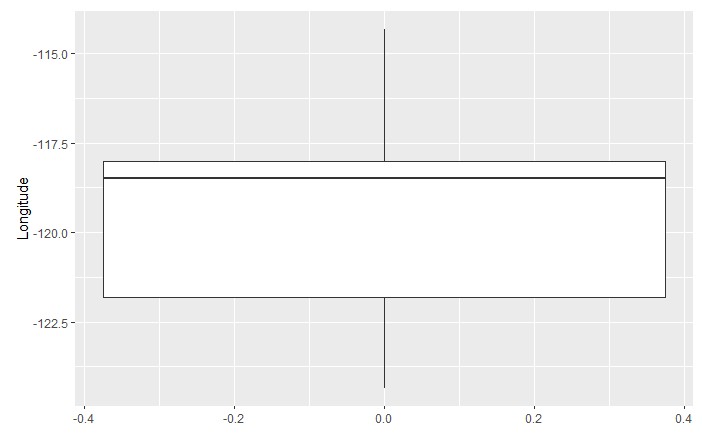
\includegraphics[width=0.7\linewidth]{figures/eda_box_1}
	\caption{Diagrama de cajas Longitude}
	\label{fig:edabox1}
\end{figure}

\newpage
Efectivamente el diagrama de cajas nos muestra que los datos se concentran en una región central densa, sin presencia de outliers.\\

Observemos la distribución de los valores en más detalle en un histograma:


\begin{figure}[h!]
	\centering
	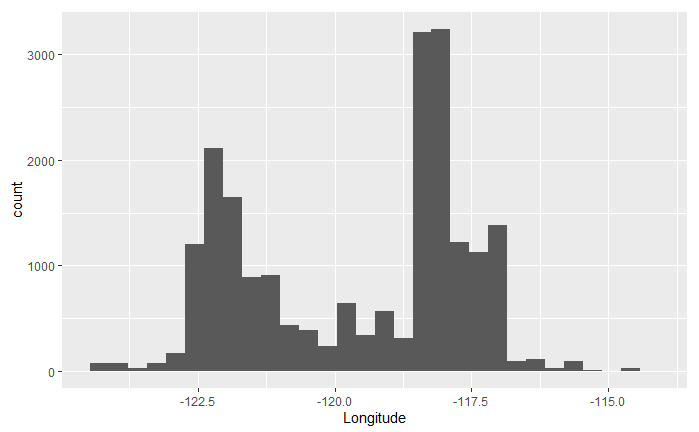
\includegraphics[width=0.7\linewidth]{figures/eda_hist_1}
	\caption{Histograma Longitude}
	\label{fig:edahist1}
\end{figure}




\newpage
	\item \textbf{Latitude}: 
	\begin{table}[h!]
		\centering
		\begin{tabular}{ll}
			& Latitude   \\
			Valor mínimo            & 32.54      \\
			Primer cuartil          & 33.93      \\
			Mediana                 & 34.26      \\
			Media                   & 35.63      \\
			Tercer cuartil          & 37.71      \\
			Valor máximo            & 41.95      \\ \hline
			Desviación estandar     & 2.135952   \\ \hline
			Coeficiente de skewness & 0.46591914 \\
			Coeficiente de Kurtosis & 1.882220  
		\end{tabular}
	\end{table}

En este caso los datos presentan una leve dispersión a la derecha, detalle que se confirma al observar una media cercana al valor del primer cuartil. De nuevo no se presenta dispersion de los datos respecto de su centro, por lo que será poco probable la existencia de outliers. \\

Se complementa este estudio con la representación gráfica de esta variable mediante un diagrama de cajas y un histograma

\begin{figure}[h!]
	\centering
	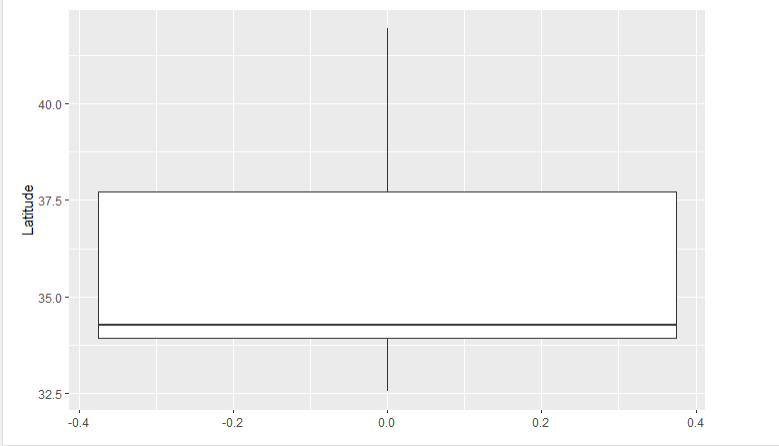
\includegraphics[width=0.7\linewidth]{figures/eda_box_2}
	\caption{Diagrama de cajas Latitude}
	\label{fig:edabox2}
\end{figure}
\newpage
\begin{figure}[h!]
	\centering
	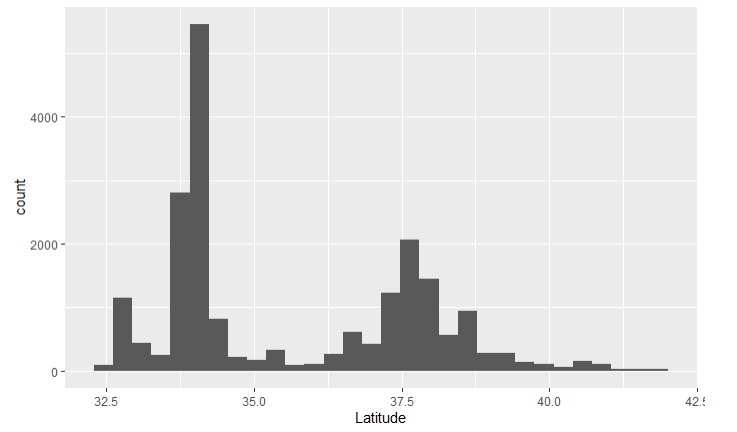
\includegraphics[width=0.7\linewidth]{figures/eda_hist_2}
	\caption{Histograma Latitude}
	\label{fig:edahist2}
\end{figure}

Se confirma una distribución concentrada de los datos levemente desplazada a valores situados a la izquierda. \\ 


	
	\item \textbf{HousingMedianAge}: 
	\begin{table}[h!]
		\centering
		\begin{tabular}{ll}
			& HousingMedianAge \\
			Valor mínimo            & 1.00             \\
			Primer cuartil          & 18.00            \\
			Mediana                 & 29.00            \\
			Media                   & 28.64            \\
			Tercer cuartil          & 37.00            \\
			Valor máximo            & 52.00            \\ \hline
			Desviación estandar     & 12.585558        \\ \hline
			Coeficiente de skewness & 0.06032625       \\
			Coeficiente de Kurtosis & 2.199274        
		\end{tabular}
	\end{table}

Los resultados estadísticos describen una variable con una región central muy densa y con una muy leve dispersión de los datos respecto a esta región central, descartando nuevamente la presencia de outliers.

Se complementa este estudio con la representación gráfica de esta variable mediante un diagrama de cajas y un histograma:
\newpage
\begin{figure}[h!]
	\centering
	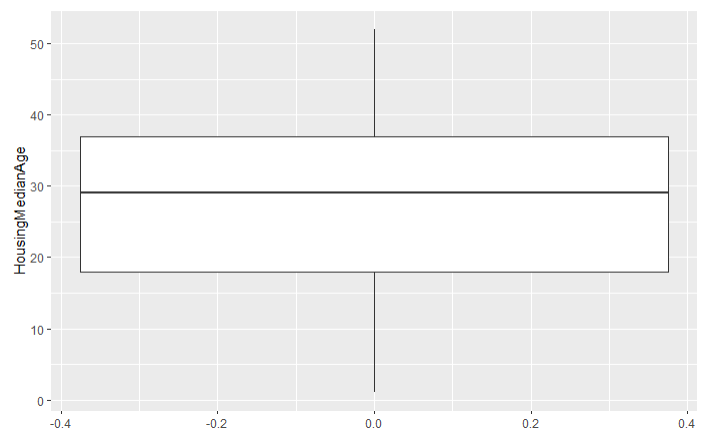
\includegraphics[width=0.7\linewidth]{figures/eda_box_3}
	\caption{Diagrama de cajas HousingMedianAge}
	\label{fig:edabox3}
\end{figure}
\begin{figure}[h!]
	\centering
	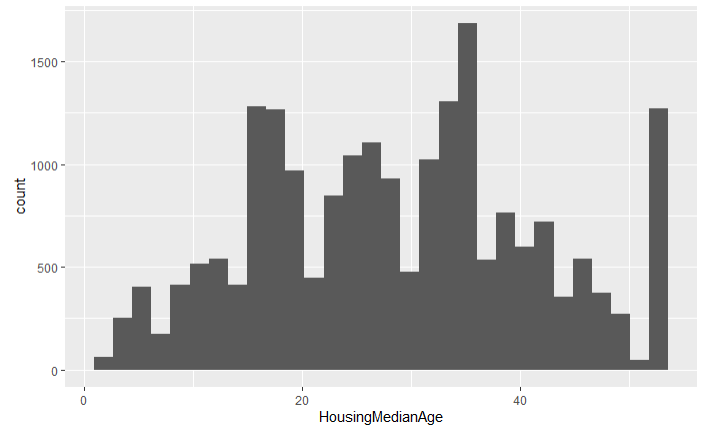
\includegraphics[width=0.7\linewidth]{figures/eda_hist_3}
	\caption{Histograma HousingMedianAge}
	\label{fig:edahist3}
\end{figure}

Se emplea el test de Shapiro-Wilk para confirmar que no se supera el nivel mínimo de significancia, y por tanto no es una distribución normal.

	
	\item \textbf{TotalRooms}: 
	\begin{table}[h!]
		\centering
		\begin{tabular}{ll}
			& TotalRooms  \\
			Valor mínimo            & 2           \\
			Primer cuartil          & 1448        \\
			Mediana                 & 2127        \\
			Media                   & 2636        \\
			Tercer cuartil          & 3148        \\
			Valor máximo            & 39320       \\ \hline
			Desviación estandar     & 2181.615252 \\ \hline
			Coeficiente de skewness & 4.14704204  \\
			Coeficiente de Kurtosis & 35.622732  
		\end{tabular}
	\end{table}


Los resultados estadísticos hacen referencia a una distribución desplazada a la izquierda. El coeficiente de Kurtosis obtenido se traduce en una amplia dispersión de los datos respecto al centro de distribución de estos, siendo en este caso, a diferencia de los anteriores, muy probable la existencia de outliers situados a la derecha.

Se complementa este estudio con la representación gráfica de esta variable mediante un diagrama de cajas y un histograma

\begin{figure}[h!]
	\centering
	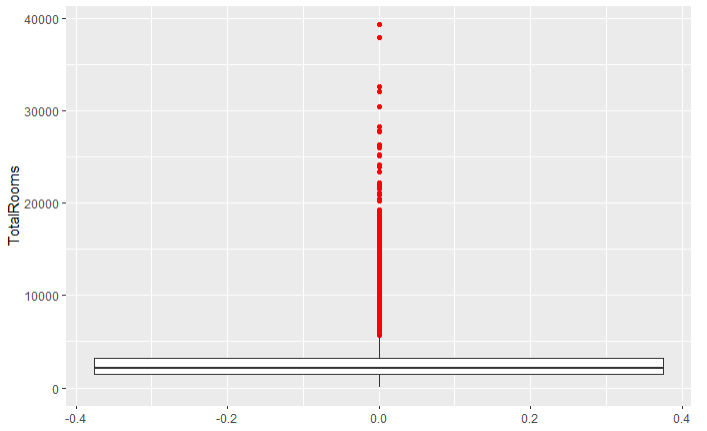
\includegraphics[width=0.7\linewidth]{figures/eda_box_4}
	\caption{Diagrama de cajas TotalRooms}
	\label{fig:edabox4}
\end{figure}
\begin{figure}[h!]
	\centering
	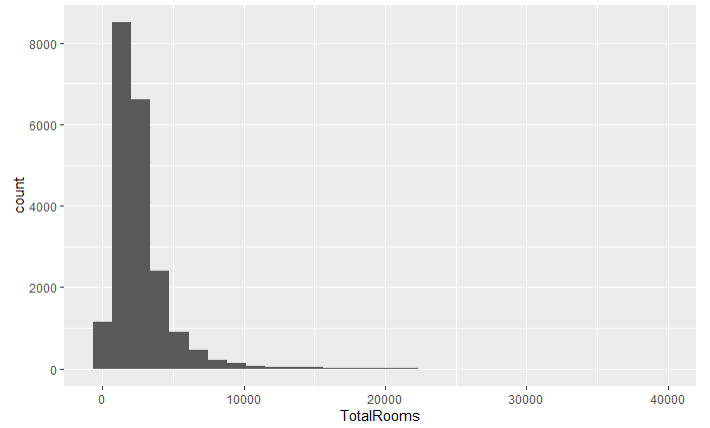
\includegraphics[width=0.7\linewidth]{figures/eda_hist_4}
	\caption{Histograma TotalRooms}
	\label{fig:edahist4}
\end{figure}


	\newpage
	\item \textbf{TotalBedrooms}: 
	\begin{table}[h!]
		\centering
		\begin{tabular}{ll}
			& TotalBedrooms \\
			Valor mínimo            & 1.0           \\
			Primer cuartil          & 295.0         \\
			Mediana                 & 435.0         \\
			Media                   & 537.9         \\
			Tercer cuartil          & 647.0         \\
			Valor máximo            & 6445.0        \\ \hline
			Desviación estandar     & 421.247906    \\ \hline
			Coeficiente de skewness & 3.45282180    \\
			Coeficiente de Kurtosis & 24.917894    
		\end{tabular}
	\end{table}

Se presenta un caso similar al anterior, en el que de nuevo el centro de la distribución se desplaza a la derecha, a la vez que se revela una amplia dispersión de los datos. 

Se complementa este estudio con la representación gráfica de esta variable mediante un diagrama de cajas y un histograma

\begin{figure}[h!]
	\centering
	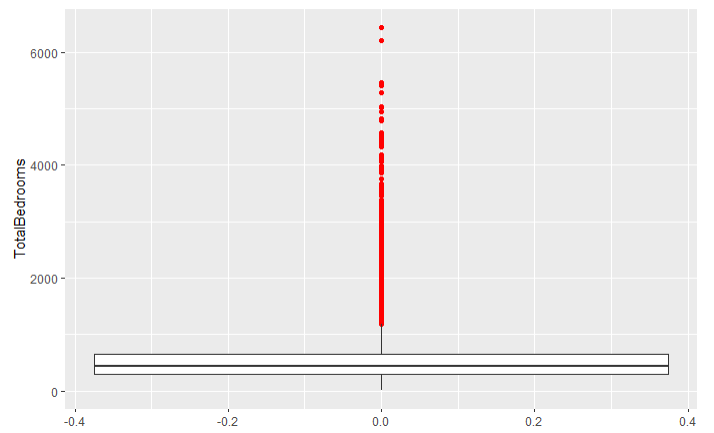
\includegraphics[width=0.7\linewidth]{figures/eda_box_5}
	\caption{Diagrama de cajas TotalBedrooms}
	\label{fig:edabox5}
\end{figure}
\newpage
\begin{figure}[h!]
	\centering
	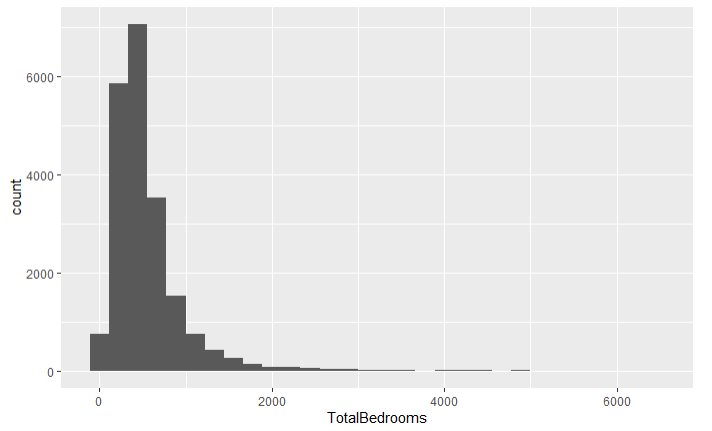
\includegraphics[width=0.7\linewidth]{figures/eda_hist_5}
	\caption{Histograma TotalBedrooms}
	\label{fig:edahist5}
\end{figure}


	
	\item \textbf{Population}: 
	\begin{table}[h!]
		\centering
		\begin{tabular}{ll}
			& Population  \\
			Valor mínimo            & 3           \\
			Primer cuartil          & 787         \\
			Mediana                 & 1166        \\
			Media                   & 1425        \\
			Tercer cuartil          & 1725        \\
			Valor máximo            & 35682       \\ \hline
			Desviación estandar     & 1132.462122 \\ \hline
			Coeficiente de skewness & 4.93549951  \\
			Coeficiente de Kurtosis & 76.535009  
		\end{tabular}
	\end{table}

Los estadísticos muestra una distribución muy estrecha, desplazada a la izquierda y con dispersión de los datos respecto de su centro, planteando la existencia de outliers.

Se complementa este estudio con la representación gráfica de esta variable mediante un diagrama de cajas y un histograma
\newpage
\begin{figure}[h!]
	\centering
	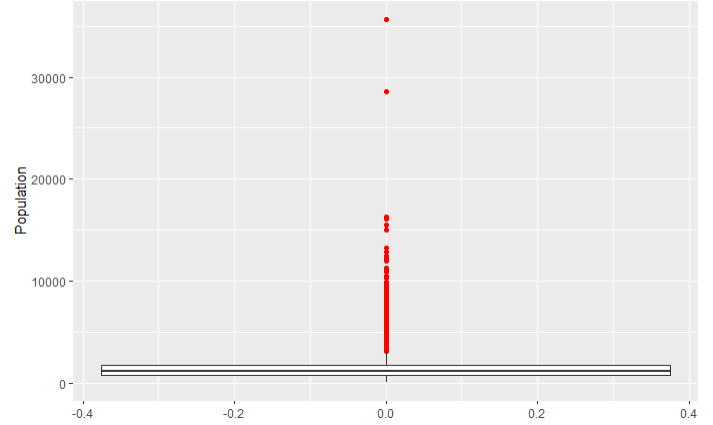
\includegraphics[width=0.7\linewidth]{figures/eda_box_6}
	\caption{Diagrama de cajas Population}
	\label{fig:edabox6}
\end{figure}
\begin{figure}[h!]
	\centering
	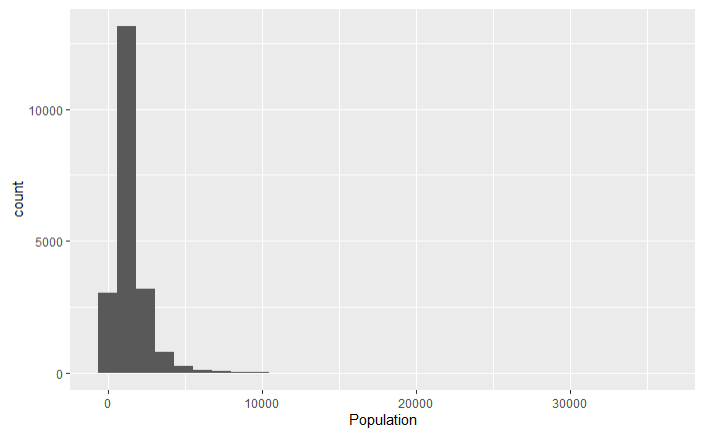
\includegraphics[width=0.7\linewidth]{figures/eda_hist_6}
	\caption{Histograma Population}
	\label{fig:edahist6}
\end{figure}

	
	\item \textbf{Households}: 
	\begin{table}[h!]
		\centering
		\begin{tabular}{ll}
			& Households \\
			Valor mínimo            & 1.0        \\
			Primer cuartil          & 280.0      \\
			Mediana                 & 409.0      \\
			Media                   & 499.5      \\
			Tercer cuartil          & 605.0      \\
			Valor máximo            & 6082.0     \\ \hline
			Desviación estandar     & 382.329753 \\ \hline
			Coeficiente de skewness & 3.41018986 \\
			Coeficiente de Kurtosis & 25.052354 
		\end{tabular}
	\end{table}

Los resultados estadísticos hacen referencia a una distribución desplazada a la izquierda con una amplia dispersión de los datos respecto al centro de distribución de estos, muy probable la existencia de outliers situados a la derecha.

Se complementa este estudio con la representación gráfica de esta variable mediante un diagrama de cajas y un histograma

\begin{figure}[h!]
	\centering
	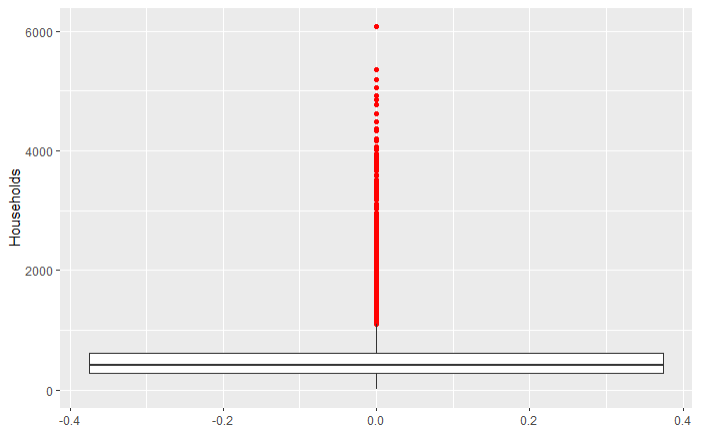
\includegraphics[width=0.7\linewidth]{figures/eda_box_7}
	\caption{Diagrama de cajas Households}
	\label{fig:edabox7}
\end{figure}
\begin{figure}[h!]
	\centering
	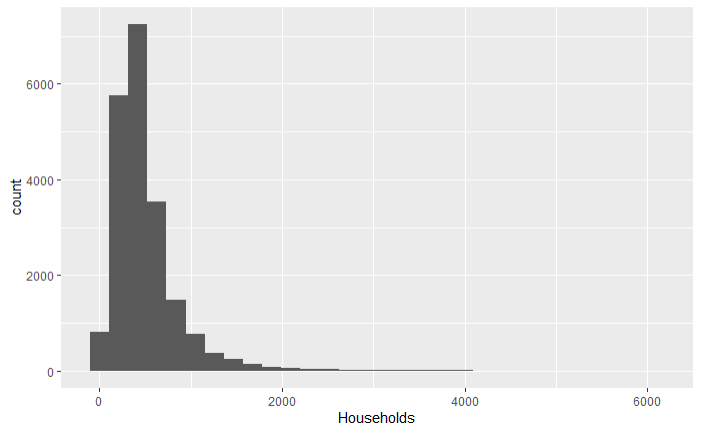
\includegraphics[width=0.7\linewidth]{figures/eda_hist_7}
	\caption{Histograma Households}
	\label{fig:edahist7}
\end{figure}

	\newpage
	\item \textbf{MedianIncome}: 
	\begin{table}[h!]
		\centering
		\begin{tabular}{ll}
			& MedianIncome \\
			Valor mínimo            & 0.4999       \\
			Primer cuartil          & 2.5634       \\
			Mediana                 & 3.5348       \\
			Media                   & 3.8707       \\
			Tercer cuartil          & 4.7432       \\
			Valor máximo            & 15.0001      \\ \hline
			Desviación estandar     & 1.899822     \\ \hline
			Coeficiente de skewness & 1.64653703   \\
			Coeficiente de Kurtosis & 7.951034    
		\end{tabular}
	\end{table}

De nuevo los datos se encuentran ligeramente desplazados a la izquierda, siendo en este caso leve la dispersión de valores respecto al centro de la distribución, revelando la existencia de outliers.

Se complementa este estudio con la representación gráfica de esta variable mediante un diagrama de cajas y un histograma

\begin{figure}[h!]
	\centering
	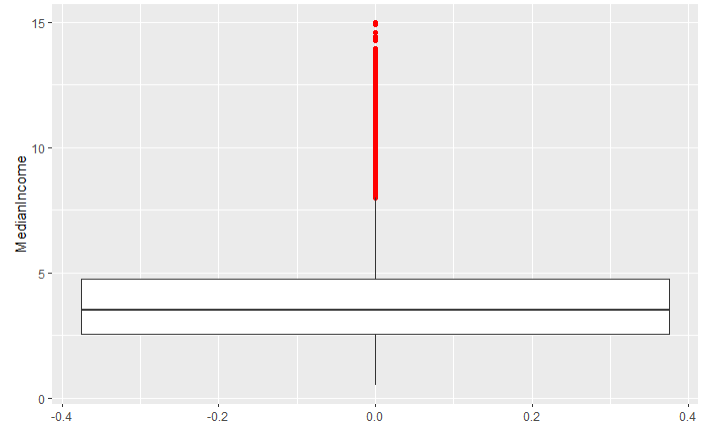
\includegraphics[width=0.7\linewidth]{figures/eda_box_8}
	\caption{Diagrama de cajas MedianIncome}
	\label{fig:edabox8}
\end{figure}
\newpage
\begin{figure}[h!]
	\centering
	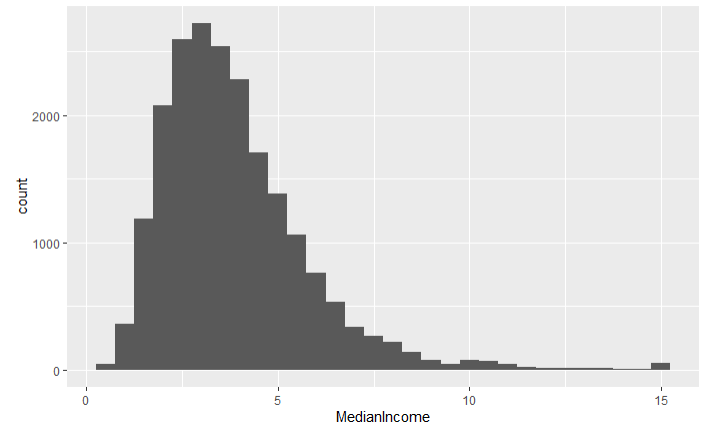
\includegraphics[width=0.7\linewidth]{figures/eda_hist_8}
	\caption{Histograma MedianIncome}
	\label{fig:edahist8}
\end{figure}


Se observa que el salario de las personas posee una distribución más o menos normal, pero con la existencia de personas con un salario más elevado que el resto, originando outliers.\\


	
\end{itemize}

Mencionar que aunque se ha indicado en cada variable que no se posee una distribución normal, esta suposición se ha confirmado realizando el test Shapiro-Wilk, el cual efectivamente no ha superado un valor por encima del nivel de significancia para ninguna de las variables, todas poseen un p-value menor a 2.2e-16. \\


Finalicemos analizando la variable dependiente, \textbf{MedianHouseValue}:
\begin{table}[h!]
	\centering
	\begin{tabular}{ll}
		& MedianHouseValue \\
		Valor mínimo            & 14999            \\
		Primer cuartil          & 119600           \\
		Mediana                 & 179700           \\
		Media                   & 206856           \\
		Tercer cuartil          & 264725           \\
		Valor máximo            & 500001           \\ \hline
		Desviación estandar     & 115395.615874    \\ \hline
		Coeficiente de skewness & 0.97769221       \\
		Coeficiente de Kurtosis & 3.327500        
	\end{tabular}
\end{table}

Se complementa este estudio con la representación gráfica de esta variable mediante un diagrama de cajas y un histograma:
\newpage

\begin{figure}[h!]
	\centering
	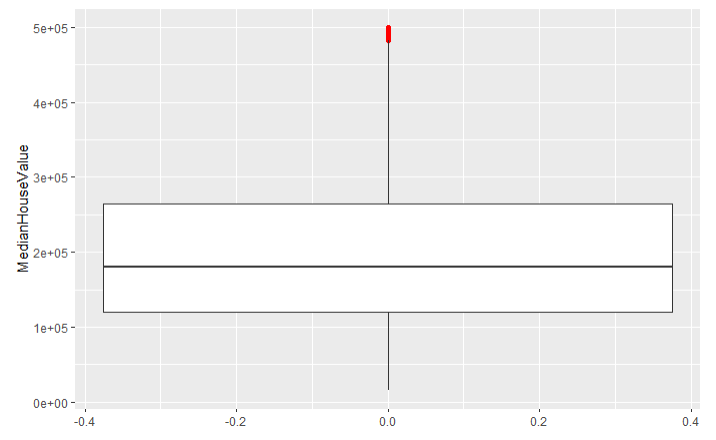
\includegraphics[width=0.7\linewidth]{figures/eda_box_9}
	\caption{Diagrama de cajas MedianHouseValue}
	\label{fig:edabox9}
\end{figure}
\begin{figure}[h!]
	\centering
	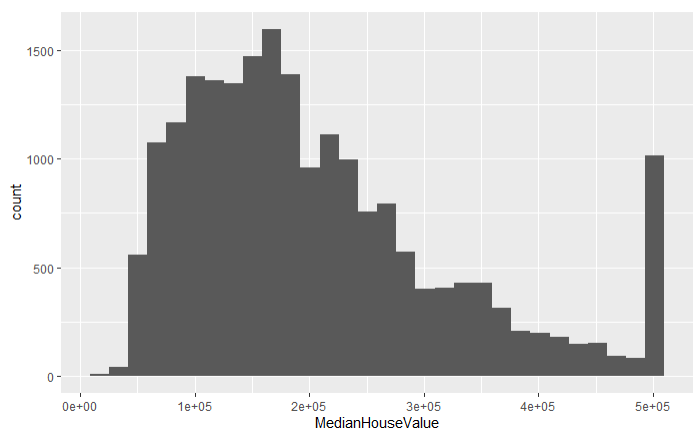
\includegraphics[width=0.7\linewidth]{figures/eda_hist_9}
	\caption{Histograma MedianHouseValue}
	\label{fig:edahist9}
\end{figure}

Se observa que la distribución de la variable dependiente posee una región central muy densa y con una leve dispersión de los datos respecto a esta. Se observa un efecto de umbral para aquellas viviendas con un valor muy elevado, ya que todas las viviendas con un valor superior a 500000 han sido fijadas en esta cantidad. \\

Comparando el valor medio de la vivienda con la media de ingresos se observa con claridad este problema:
\newpage
\begin{figure}[h!]
	\centering
	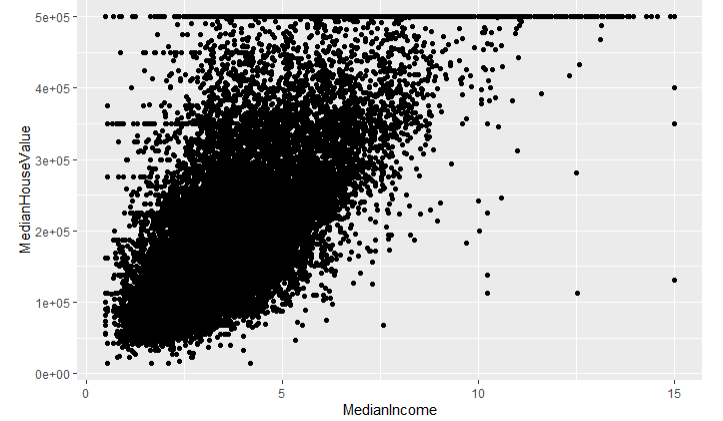
\includegraphics[width=0.7\linewidth]{figures/truncado}
	\caption{}
	\label{fig:truncado}
\end{figure}

Todos estos casos poseen un valor asignado incorrecto y por ello se procede a su eliminación, con el objetivo de evitar que estos afecten en la posterior generación de modelos. Por suerte estos casos representan un porcentaje muy bajo de los datos (sobre 1\%).

\begin{figure}[h!]
	\centering
	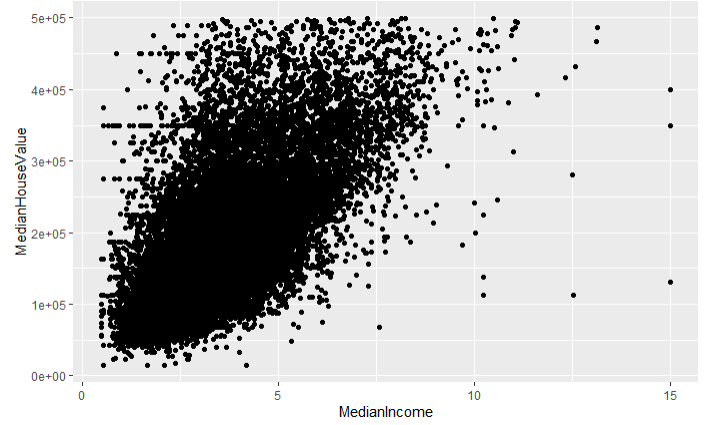
\includegraphics[width=0.7\linewidth]{figures/post-truncado}
	\caption{}
	\label{fig:post-truncado}
\end{figure}



Este paso reduce el número de outliers pero aún así se estudiaran en el siguiente apartado en aquellas variables que he considerado de estudio.

\newpage
\subsection{Análisis de valores anómalos}
Nos fijamos en los atributos anteriores en los que se presentaron valores outliers:

\begin{figure}[!tbh]
	\centering
	\begin{subfigure}{0.5\textwidth}
		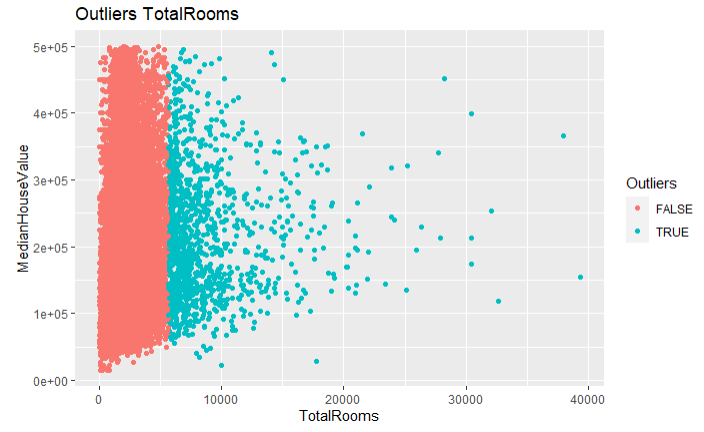
\includegraphics[width=1\linewidth]{figures/out_1}
		\caption{}
		\label{fig:out1}
	\end{subfigure}\hfil % <-- added
	\begin{subfigure}{0.5\textwidth}
		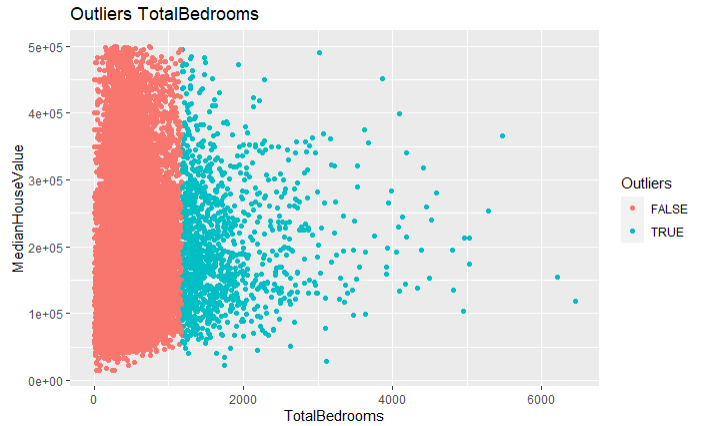
\includegraphics[width=1\linewidth]{figures/out_2}
		\caption{}
		\label{fig:out2}
	\end{subfigure}\hfil % <-- added
	
	\medskip
	
	\begin{subfigure}{0.5\textwidth}
		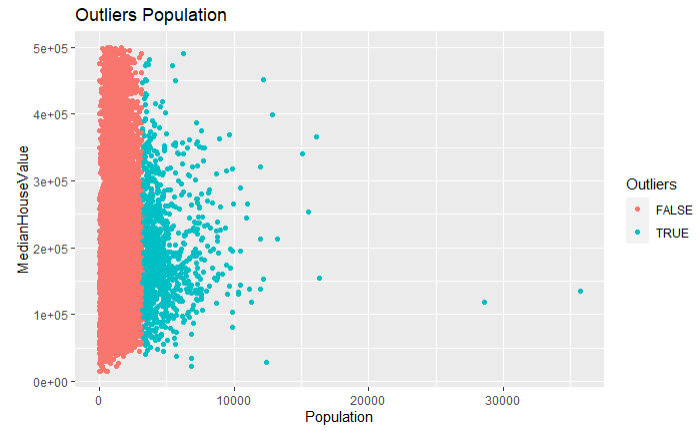
\includegraphics[width=1\linewidth]{figures/out_3}
		\caption{}
		\label{fig:out3}
	\end{subfigure}\hfil % <-- added
	\begin{subfigure}{0.5\textwidth}
		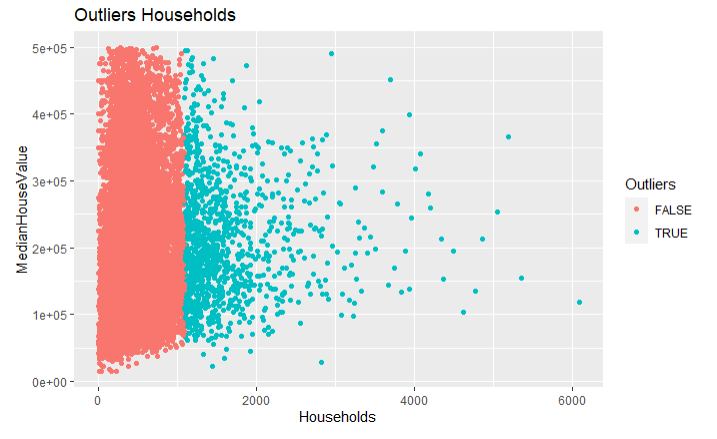
\includegraphics[width=1\linewidth]{figures/out_4}
		\caption{}
		\label{fig:out4}
	\end{subfigure}\hfil % <-- added

	\medskip
		\begin{subfigure}{0.5\textwidth}
	\centering
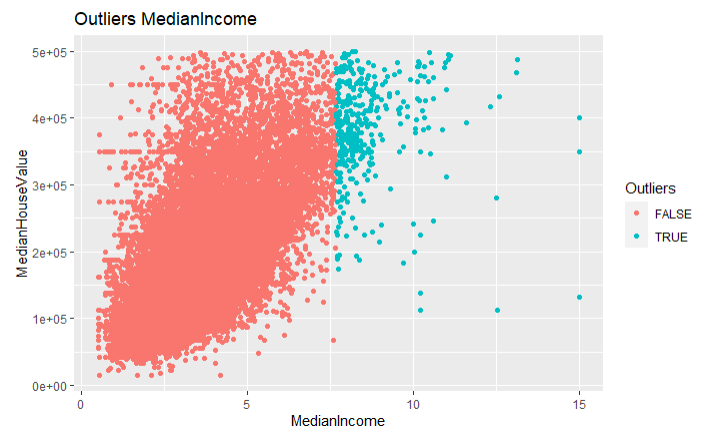
\includegraphics[width=1\linewidth]{figures/out_5}
\caption{}
\label{fig:out5}
	\end{subfigure}\hfil % <-- added
	
	\caption{Outliers California}
	\label{PCA_A}
\end{figure}





Nos fijamos solo en los casos cuyo valor del tercer cuartil más 1.5 veces su rango intercuartil, casos que son considerados como outliers extremos. Efectivamente se detectan numerosos casos que influirán de manera negativa en la realización de los modelos. Al tratarse de un 6\% del total de los datos, un porcentaje muy bajo, pues tenemos un dataset muy denso, he decidido que su eliminación será una ventaja.




\newpage
\section{Análisis de las relaciones entre variables}
Conocidas en profundidad cada una de las variables, el próximo paso es el estudio de las posibles relaciones existentes entre ellas. Este estudio tendrá como objetivo determinar si existe un alto nivel de dependencia entre algunas de las variables, detalle que debe ser tenido en cuando en el posterior proceso de elaboración de modelos.\\

El siguiente diagrama de correlaciones permite efectuar este estudio entre cada par de variables que forman el dataset. Las correlación es entre cada una de ellas s calcula gracias al test de Kendall.

\begin{figure}[h!]
	\centering
	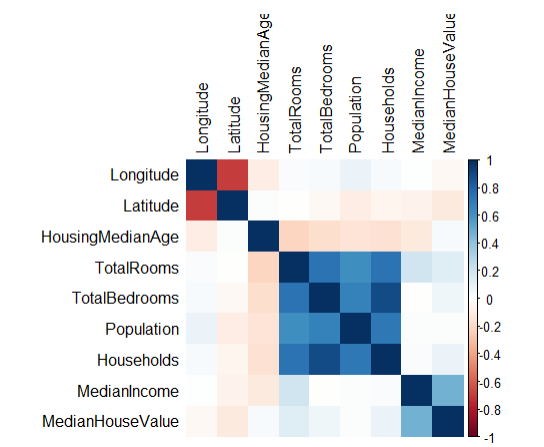
\includegraphics[width=0.7\linewidth]{figures/corre_1}
	\caption{Correlaciones California}
	\label{fig:corre1}
\end{figure}


Observando la matriz de correlación se confirman relaciones entre variables obvias y fáciles de predecir. Algunas de estas relaciones confirman que cuantos más hogares hay un bloque mayor es el número de dormitorios; de igual manera una mayor población también se vincula con un mayor número de dormitorios. Otra relación menos clara y en la que se profundiza en el siguiente apartado es en la existente relación entre la media de ingresos en el hogar con el valor medio de la vivienda.



\newpage
\section{Comprobación de hipótesis planteadas}
\textbf{California posee una amplia zona de costa permitiendo las variables de latitud y longitud determinar la cercanía de cada grupo de viviendas al mar. ¿Cómo de importante es la localización de la vivienda a la hora de determinar su precio?}

Para comprobarlo se crea un scatterplot con las variables de latitud y longitud, que utilice la variable MedianHouseValue para asignarle color a cada punto dependiendo si la media de las casas de esa zona es de un alto o bajo precio. 

\begin{figure}[h!]
	\centering
	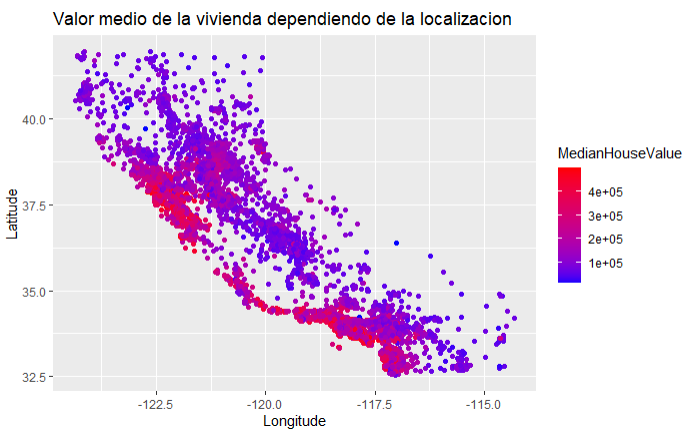
\includegraphics[width=0.7\linewidth]{figures/hipo_1}
	\caption{}
	\label{fig:hipo1}
\end{figure}

Se observa que los puntos representados pertenecen a una representación gráfica del estado de California, por ello para facilitar la compresión de los resultados se haya un mapa de este estado.

\begin{figure}[h!]
	\centering
	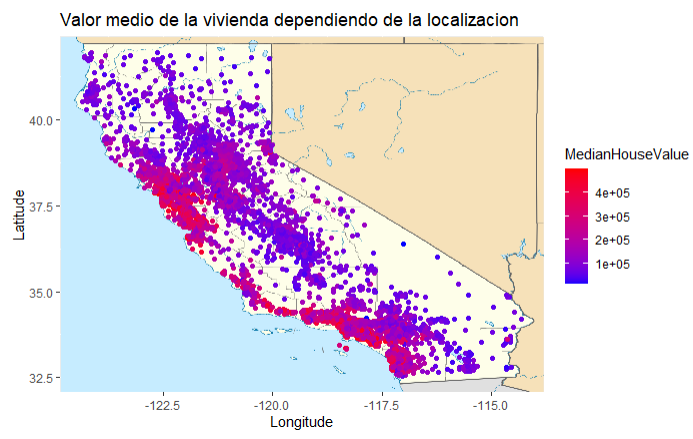
\includegraphics[width=0.7\linewidth]{figures/hipo_2}
	\caption{}
	\label{fig:hipo2}
\end{figure}

Efectivamente observamos que prácticamente todas las casas de alto valor se encuentran relativamente cerca del mar, resaltando la importancia de la proximidad a la costa en el análisis. 
Pero existe una excepción y se trata de la zona norte de California, donde a pesar de la cercanía al océano las viviendas no poseen un valor elevado. Tras investigar las diferentes ciudades de California he determinado que esto puede ser causado porque las principales ciudades de california se sitúan en la zona de costa central y sur. En la siguiente hipótesis se estudiará en más detalle esta observación.



\vspace{1cm}
\textbf{En ocasiones zonas con menos densidad de población suele estar relacionado con poblaciones más privilegiadas, ¿el precio de la vivienda tendrá una alta relación con la densidad de la población?}

De nuevo para facilitar la compresión de los resultados se efectuarán las gráficas sobre un mapa de California.


\begin{figure}[!tbh]
	\centering
	\begin{subfigure}{0.5\textwidth}
		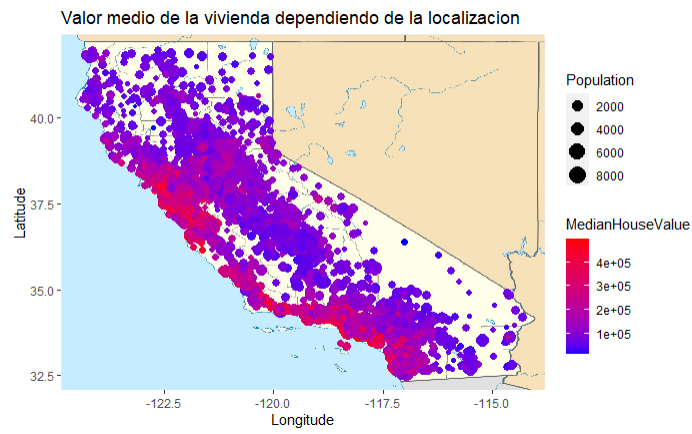
\includegraphics[width=1\linewidth]{figures/hipo_3}
		\caption{}
		\label{fig:hipo3}
	\end{subfigure}\hfil % <-- added
	\begin{subfigure}{0.5\textwidth}
		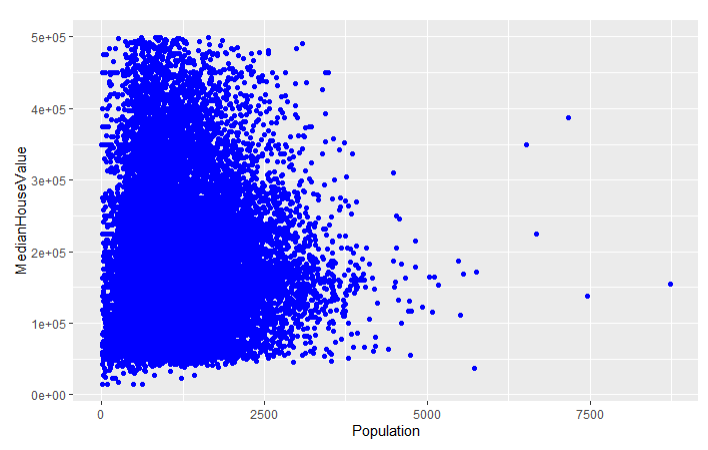
\includegraphics[width=1\linewidth]{figures/hipo_4}
		\caption{}
		\label{fig:hipo4}
	\end{subfigure}\hfil % <-- added
\end{figure}

Observamos que a pesar de que la capital de Callifornia sea Sacramento, situada en aproximadamente Latitud 38 y longitud -122, siendo una de las zonas con mayor población, la mayoría de los bloques situados en ella contienen casas de bajo presupuesto. Además se observa que cuanto más nos acercamos a regiones de montañas (centro/oeste) las poblaciones son más pequeñas al igual que el precio de la vivienda.\\

Investigando la geografía de California determino que aquellas concentraciones de viviendas de gran precio situadas en la costa corresponden a las grandes ciudades de este Estado, como son San Francisco, Los Ángeles, San Diego o San Jose. 



\newpage
\textbf{La variable MedianIncome indica los ingresos medios de los hogares, ¿posee esta una fuerte relación positiva con el valor de la vivienda?}

Nos apoyamos en un scatterplot para observar la relación entre estas dos variables.

\begin{figure}[h!]
	\centering
	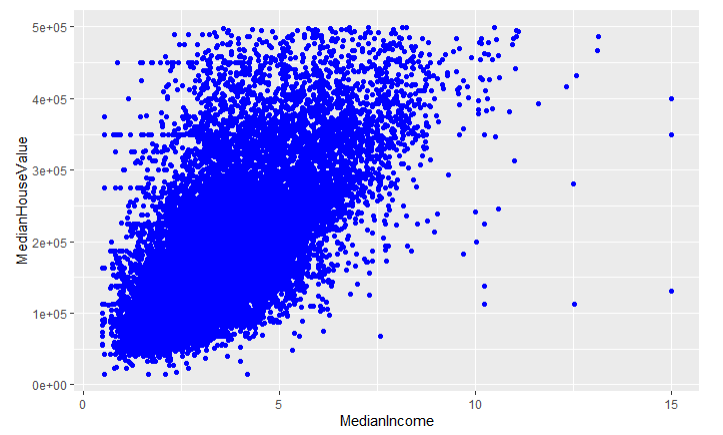
\includegraphics[width=0.7\linewidth]{figures/hipo_5}
	\caption{}
	\label{fig:hipo5}
\end{figure}

Se observa una fuerte relación entre estas variables, en la que efectivamente una media de ingresos elevados suele ir vinculada con viviendas de mayor precio. Esta relación será importante en la posterior creación de modelos de regresión.



\newpage
\textbf{Un factor interesante de estudio es la antigüedad de la vivienda, lo esperable sería que una casa nueva tuviera mayor precio que una antigua. Lo lógico es pensar que una casa nueva tenga mayor valor que una vieja.}


\begin{figure}[!tbh]
	\centering
	\begin{subfigure}{0.5\textwidth}
	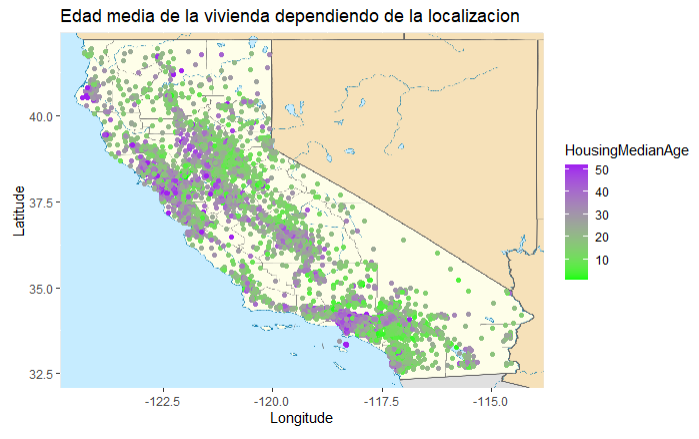
\includegraphics[width=1\linewidth]{figures/hipo_6}
\caption{}
\label{fig:hipo6}
	\end{subfigure}\hfil % <-- added
	\begin{subfigure}{0.5\textwidth}
	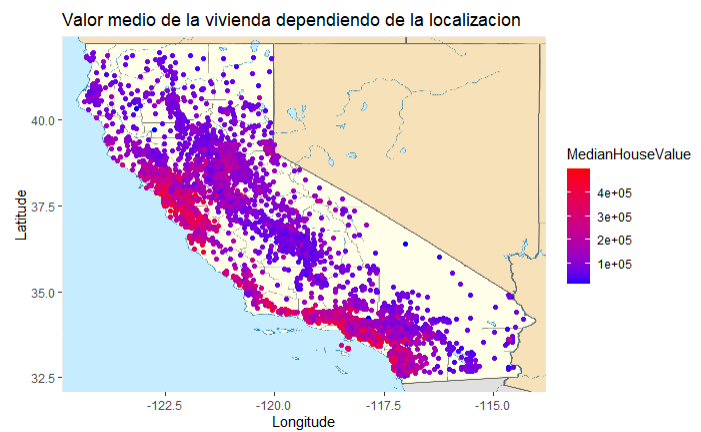
\includegraphics[width=1\linewidth]{figures/hipo_7}
\caption{}
\label{fig:hipo7}
	\end{subfigure}\hfil % <-- added
\end{figure}



Comparando los dos mapas llegamos a la conclusión de que cuanto más vieja la casa más cara es esta, algo que de primeras no parece tener sentido. Sin embargo, como ya hemos descubierto previamente, las viviendas en la costa tienen mayor precio, siendo de nuevo este el factor de mayor impacto en el dataset, junto con el ingreso de dinero en cada domicilio.\\

Podemos concluir en que cuanto más nueva sea la casa mayor será la probabilidad de que esta se ubique en una zona no costera, en el interior. 



